% Этот шаблон документа разработан в 2014 году
% Данилом Фёдоровых (danil@fedorovykh.ru) 
% для использования в курсе 
% <<Документы и презентации в \LaTeX>>, записанном НИУ ВШЭ
% для Coursera.org: http://coursera.org/course/latex .
% Исходная версия шаблона --- 
% https://www.writelatex.com/coursera/latex/3.2

\documentclass[a4paper,final,14pt]{article}

%%% Работа с русским языком
\usepackage{cmap}					% поиск в PDF
\usepackage{mathtext} 				% русские буквы в фомулах
\usepackage[T2A]{fontenc}			% кодировка
\usepackage[utf8]{inputenc}			% кодировка исходного текста
\usepackage[english,russian]{babel}	% локализация и переносы

%%% Дополнительная работа с математикой
\usepackage{amsmath,amsfonts,amssymb,amsthm,mathtools} % AMS
\usepackage{icomma} % "Умная" запятая: $0,2$ --- число, $0, 2$ --- перечисление

%% Свои команды
%% Перенос знаков в формулах (по Львовскому)
\newcommand*{\hm}[1]{#1\nobreak\discretionary{}
{\hbox{$\mathsurround=0pt #1$}}{}}

%%% Работа с картинками
% \usepackage{graphicx}  % Для вставки рисунков
% \graphicspath{{images/}{images2/}}  % папки с картинками
% \setlength\fboxsep{3pt} % Отступ рамки \fbox{} от рисунка
% \setlength\fboxrule{1pt} % Толщина линий рамки \fbox{}
% \usepackage{wrapfig} % Обтекание рисунков текстом

%%% Работа с таблицами
\usepackage{array,tabularx,tabulary,booktabs} % Дополнительная работа с таблицами
\usepackage{longtable}  % Длинные таблицы
\usepackage{multirow} % Слияние строк в таблице
%%% Теоремы
\theoremstyle{plain} % Это стиль по умолчанию, его можно не переопределять.
\newtheorem{theorem}{Теорема}[section]
\newtheorem{proposition}[theorem]{Утверждение}
 
\theoremstyle{definition} % "Определение"
\newtheorem{corollary}{Следствие}[theorem]
\newtheorem{problem}{Задача}[section]
 
\theoremstyle{remark} % "Примечание" \newtheorem*{nonum}{Решение}
%%% Программирование
\usepackage{etoolbox} % логические операторы

%%% Страница
\usepackage{extsizes} % Возможность сделать 14-й шрифт
% \usepackage{geometry} % Простой способ задавать поля
% 	\geometry{top=25mm} \geometry{bottom=35mm}
% 	\geometry{left=35mm}
% 	\geometry{right=20mm}
 %
\usepackage{setspace}
\usepackage{indentfirst}
\usepackage{geometry}
\geometry{
  a4paper,
  left=20mm,top=15mm,right=20mm,bottom=15mm,
  headheight=0pt,headsep=0mm,foot=0pt,footskip=13mm,
  includeheadfoot
}
\linespread{1.05}
\raggedbottom
\sloppy


\usepackage{setspace} % Интерлиньяж
%\onehalfspacing % Интерлиньяж 1.5
%\doublespacing % Интерлиньяж 2
%\singlespacing % Интерлиньяж 1

\usepackage{lastpage} % Узнать, сколько всего страниц в документе.

\usepackage{soul} % Модификаторы начертания

\usepackage{hyperref} \usepackage[usenames,dvipsnames,svgnames,table,rgb]{xcolor}
\hypersetup{				% Гиперссылки
    unicode=true,           % русские буквы в раздела PDF
    pdftitle={Ответы на экзамен по матанализу},   % Заголовок
    pdfauthor={Кутузов Дмитрий},      % Автор
    pdfsubject={Матанализ},      % Тема
    pdfcreator={Кутузов Дмитрий Николаевич}, % Создатель
    pdfproducer={Кутузов Дмитрий Николаевич}, % Производитель
    pdfkeywords={матан} {матанализ} {математический анализ}, % Ключевые слова
    colorlinks=true,       	% false: ссылки в рамках; true: цветные ссылки
    linkcolor=red,          % внутренние ссылки
    citecolor=green,        % на библиографию
    filecolor=magenta,      % на файлы
    urlcolor=cyan           % на URL
}

%\renewcommand{\familydefault}{\sfdefault} % Начертание шрифта

\usepackage{multicol} % Несколько колонок

\author{Кутузов Дмитрий}
\title{Ответы на билеты по математическому анализу}
\date{\today}


% \usepackage{lmodern}         % for the looks
\usepackage{tikz}            % the graphics
\usepackage{textcomp}        % for \textregistered

\begin{document} % конец преамбулы, начало документа

\thispagestyle{empty}

\definecolor{mycyan}{RGB}{201, 212, 255}
\definecolor{myblack}{RGB}{22, 26, 30}

\begin{tikzpicture}[remember picture,overlay]

\node [align=center] at (current page.north) % upper
      {\begin{tikzpicture}[remember picture, overlay]
	  \fill[fill=mycyan] (-10,0) rectangle (10,-0.5);
	  \node[anchor=north] at (0,-0.5) {\Large\textit{Независимое учебное издание}};
      \end{tikzpicture}};
      
\node [align=center] at (current page.center) % dragon
      {\begin{tikzpicture}[remember picture, overlay]
          \node[anchor=center,align=center] at (0,3)
               {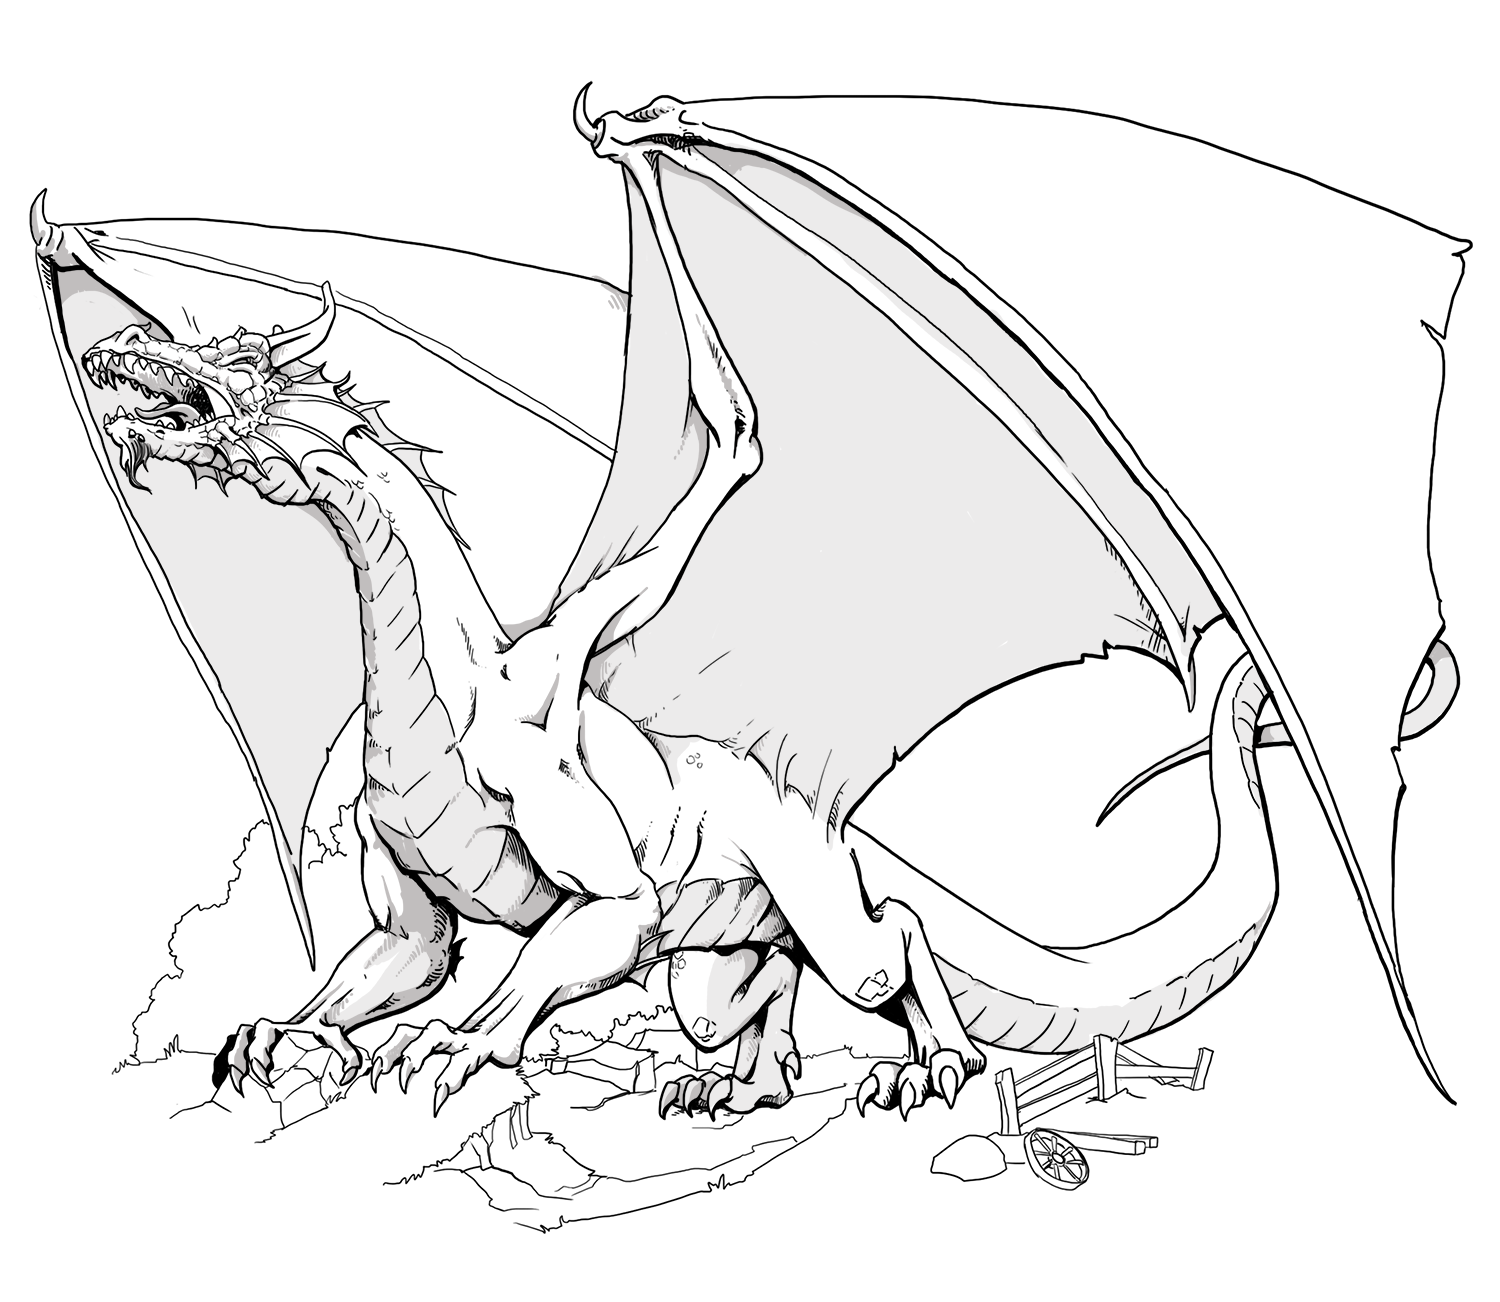
\includegraphics[width=1.2\textwidth]{dragon.png}};
               % from https://commons.wikimedia.org/wiki/File:DnD_Dragon.png
      \end{tikzpicture}};

\node [yshift=-5cm] at (current page.center) % title
      {\begin{tikzpicture}[remember picture, overlay]
          \fill[fill=mycyan] (-10,-4) rectangle (10 ,0);
          \node[align=center] at (0,-2)
               {\resizebox{1.1\linewidth}{!}{\Huge\textbf{Математический анализ}}};
	       \node[anchor=east,align=right] at (10,-5.5) {\Huge\color{black}\textit{Экзамен 2 семестра}};
      \end{tikzpicture}};

\node [shift={(-5cm,-5cm)}] at (current page.north east) % Revision 2
      {\begin{tikzpicture}[remember picture, overlay]
          \draw[fill=myblack] (0,5) -- (1.5,5) -- (5,1.5) -- (5,0) -- cycle ;
          \node[inner sep=0pt,rotate=-45] (rev) at (2.9,2.9) {\huge\color{white}\textbf{Издание 1}};
      \end{tikzpicture}};

\node [align=center] at (current page.south) % bottom
      {\begin{tikzpicture}[remember picture, overlay]
          \node[anchor=south west, align=left] at (-10,0.5)
               {\resizebox{.3\linewidth}{!}
                 {\Huge\color{black}
                   \textbf{HSE NN 21ПИ}}};
               \node[anchor=south east, align=right] at (10,0.5) {\huge\color{black}\textbf{Дмитрий Кутузов}};
      \end{tikzpicture}};

\end{tikzpicture}

\newpage

Главный редактор -- Кутузов Д.Н.

\vspace{5mm}

Отдельная благодарность контрибьюторам и друзьям, которые меня поддерживали:
\begin{itemize}
  \item Хадиев Э.И.
  \item Pasha831
  \item StasRomanov
\end{itemize}

\vspace{10mm}

\textit{Данная книжка создана с целью облегчения подготовки к экзамену по
	математическому анализу 1 курса Программной Инженерии Высшей
	Школы Экономики в г. Нижний Новгород. В ней присутствуют
	большинство теорем с доказательством, которые читает лектор. Книжка
  содержит материал по курсу с 1.01.2022г. \textbf{Копирование в личных, в том числе и коммерческих целях, a также распространение в сети интернет запрещено.}}

\vspace{5mm}


\newpage


{
	\hypersetup{linkcolor=blue}
	\tableofcontents
	\newpage
}


\section*{Дифференцируемость и непрерывность функций одной переменной.}
\addcontentsline{toc}{section}{Производные высших порядков, правила их вычисления.}


\subsection*{Производные высших порядков, правила их вычисления.}
\addcontentsline{toc}{subsection}{Производные высших порядков, правила их вычисления.}

Пусть $f: X \rightarrow \mathbf{R}$, $x_o$ - внутренняя точка области определения $X$, и пусть в некоторой окрестности $U(x_0)$ точки $x_0$ везде существует производная. Тогда в окрестности $U(x_0)$ определена функция $\phi(x) = f'(x)$, поэтому $x_0$ - внутренняя точка области определения функции $\phi$. Значит в этой точке определена производная для функции $\phi$, называемая второй производной функции $f$ (или производной второго порядка) в точке $x_0$:

\[
	f''(x) = \phi'(x_0) \text{, или } f''(x_0) = (f')'(x_0)
\]

Аналогично определяется производная третьего, четвертого порядка и так далее:

\[
	f'''(x_0) = (f'')'(x_0)
\]
\[
	f^{(4)}(x_0) = (f''')'(x_0)
\]
\[
	...
\]
\[
	f^{(n)}(x_0) = (f^{(n-1)})'(x_0)
\]

\textbf{Правила вычисления производных высших порядков}

\[
	(c \cdot f)^{(n)} = c \cdot f^{(n)}
\]

\[
	(f + g)^{(n)} = f^{(n)} + g^{(n)}
\]

\[
	(f \cdot g)^{(n)} = \sum_{k = 0}^{n} C_n^k \cdot f^{(n-k)} \cdot g^{(k)}
\]


\newpage
\subsection*{Производная от функции, заданной параметрически.}
\addcontentsline{toc}{subsection}{Производная от функции, заданной параметрически.}

Говорят, что функция $y(x)$ задана параметрически, если и переменная $x$, и функция $y$ заданы как функции некоторого параметра $t$:

\[
	y(x) =
	\begin{cases}
		x = x(t) \\
		y = y(t)
	\end{cases} t\in T
\]

Однако чаще всего найти явное выражение для $y(x)$ сложно или невозможно. Как считать производную функции, заданной параметрически, когда нельзя выразить функцию явно?

Из формулы вычисления дифференциала \[ dy = y'(x) \cdot dx \] учитывая равенства $ dx = x'(t) \cdot dt $ и $ dy = y'(t) \cdot dt $ получаем \[ y'(x) = \frac{dy}{dx} = \frac{y'(t) \cdot dt}{x'(t) \cdot dt} = \frac{y'(t)}{x'(t)} \]

Вторая производная $y''(x) = (y'(x))'$:
\[
	y''(x) = \frac{(y'(x))'_t}{x'_t} = \frac{1}{x'_t} \cdot \left( \frac{y'(t)}{x'(t)} \right)'_t
\]

или

\[
	\frac{d^2y}{dx^2} = y''_{xx} = (y'_x)' = \frac{dy'_x}{dx} = \frac{(y'_x)'_t}{x'_t}
\]

\newpage
\subsection*{Производная от функции, заданной неявно.                                                   }
\addcontentsline{toc}{subsection}{Производная от функции, заданной неявно. }

Неявное задание - один из способов задания функциию Функция задана явно, если она задана уравнением $y = y(x)$. Уравнение $F(x, y) = 0$ задает функцию $y(x)$ неявно. Одну и ту же функцию можно задать разными способами (например уравнение окружности)

\textbf{Как считать производную функции заданной неявно}

Нужно равенство $F(x, y) = 0$ дифференцировать как тождество, считая $x$ независимой переменной, а $y$ - функцией от $x$



\newpage
\subsection*{Дифференциалы высших порядков и их свойства.                                               }
\addcontentsline{toc}{subsection}{Дифференциалы высших порядков и их свойства. }
\textit{\textbf{Определение:}} Дифференциал второго порядка - это дифференциал от дифференциала первого порядка:
\[
	d^2y = d(dy)
\]

\textbf{\textit{Выведем формулу для вычисления дифференциала второго порядка.}}

Дифференциал первого порядка вычисляется по формуле
\[
	dy = y'(x) dx
\]

Дифференциал первого порядка - это функция от двух переменных: $x$ и приращения $dx$.

Зафиксируем $dx$, будем считать, что меняется только переменная $x$.

Подставляя в формулу $d^2y = d(dy)$ для второго дифференциала формулу для вычисления первого $dy = y'(x)dx$ и пользуясь правилами вычисления дифференциала, получаем
\[
	d^2y = d(y'(x) \cdot dx) = (y'(x)dx)'dx = y''(x)(dx)^2
\]

Итак, получили формулу для вычисления дифференциала второго порядка:

\[
	d^2y = y''(x) \cdot dx^2
\]

Аналогично выводится формула для вычисления дифференциала $n$-го порядка:
\[
	d^ny = y^{(n)}dx^n
\]

\textbf{Свойства дифференциала порядка $n$:}

\[
	d^n(c\cdot f) = c\cdot d^n f
\]
\[
	d^n(f + g) = d^nf + d^ng
\]
\[
	d^n(f\cdot g) = \sum_{k = 0}^n C_n^k \cdot d^{n-k}f \cdot d^k g
\]

Свойство инвариантности, справедливое для дифференциала первого порядка, для дифференциала $n$ порядка в общем случае не выполняется. Действительно, пусть переменная $x$ является функцией от новой переменной $x = x(t)$.

Тогда пользуясь правилом для вычисления дифференциала от произведения, получим:
\[
	d^2y = d(y'(x)dx) = d(y'(x)) \cdot dx + y'(x) \cdot d^2x
\]
\[
	d^2y = y''(x) \cdot dx^2 + y'(x) \cdot x''_t dt^2
\]

Формулы (1) и (2) отличаются вторым слагаемым. Если оно не равно нулю, то свойство инвариантности дифференциала 2-го порядка не выполняется. Второе слагаемое обращается в нуль в том случае, если функция $x(t)$ линейна. Поэтому при линейной замене $x(t) = at + b$ свойство инвариантности дифференциала 2-го (и n-го) порядка верно.




\newpage
\subsection*{Теорема Ферма.                                                                             }
\addcontentsline{toc}{subsection}{Теорема Ферма. }

Пусть выполняются следующие условия:

\begin{enumerate}
	\item Функция определена на промежутке $X$
	\item $x_0$ - внутренняя точка промежутка $X$
	\item функция в точке $x_0$ принимает наибольшее значение, т.е. $f(x) \leq f(x_0)$ для всех точек из промежутка $X$
	\item Существует конечная производная в точке $x_0$
\end{enumerate}
\[ \textbf{Тогда } f'(x_0) = 0 \]

\textit{\textbf{Замечание:}} Теорема также верна, если функция в точке $x_0$ принимает наименьшее значение.

\textit{\textbf{Доказательство:}}

\[
	f'(x_0) = \lim_{\Delta x \rightarrow 0} \frac{f(x_0 + \Delta x) - f(x_0)}{\Delta x} = A
\]

По теории о связи существования предела и односторонних пределов:

\[
	\exists f'(x_0) = A \in \mathbf(R) \Leftrightarrow \exists f'_-(x_0) = f'_+(x_0) = A
\]

\[
	f'_-(x_0) = f'_+(x_0) = \lim_{\Delta x \rightarrow 0 + 0} \frac{f(x_0 + \Delta x) - f(x_0)}{\Delta x} = f'(x_0) = 0
\]
Что и требовалось доказать


\newpage
\subsection*{Теорема Ролля.                                                                             }
\addcontentsline{toc}{subsection}{Теорема Ролля. }

\begin{enumerate}
	\item Функция $f$ определена и непрерывна на отрезке $[a, b]$
	\item Функция $f$ дифференцируема на $(a, b)$
	\item $f(a) = f(b)$
\end{enumerate}

Тогда внутри $(a, b)$ найдется точка, в которой производная функции равна нулю:
\[
	x_0 \in (a, b): f'(x_0) = 0
\]

\textit{\textbf{Доказательство:}}

\textbf{Вторая теорема Вейерштрасса:}

Если функция определена и непрерывна на отрезке, то она достигает на нем своих точных верхней и нижней граней.

Обозначим
\[ M = sup_{x \in [a, b]}f(x); m = inf_{x \in [a, b]} f(x) \]

\begin{enumerate}
	\item $m = M: \forall x_0 \in (a, b): f(x_0) = f(a) = f(b) \Rightarrow f(x) = const \Rightarrow f'(x_0) = 0$
	\item $m < M$
\end{enumerate}

Поскольку функция на концах отрезка принимает одинаковые значения, то одно из значений (либо $m$, либо $M$) достигается во внутренней точке $x_0$.

Тогда для точки $x_0$ выполняются все условия теоремы Ферма, поэтому $f'(x_0) = 0$




\newpage
\subsection*{Теорема Лагранжа.                                                                          }
\addcontentsline{toc}{subsection}{Теорема Лагранжа. }

Пусть
\begin{enumerate}
	\item Функция $f$ определена и непрерывна на отрезке $[a, b]$
	\item Функция $f$ дифференцируема на $(a, b)$
\end{enumerate}
Тогда
\[
	\exists c \in (a, b): f'(c) = \frac{f(b) - f(a)}{b - a}
\]

\textit{\textbf{Доказательство:}}

Введем вспомогательную функцию $F(x) = f(x) - \lambda x$
\[
	F(a) = F(b): f(a) - \lambda a = f(b) - \lambda b
\]

\[
	\lambda = \frac{f(b) - f(a)}{b - a}
\]

То есть \[F(x) = f(x) - \frac{f(b) - f(a)}{b - a} \cdot x\]

Видим, что функция $F(x)$ удовлетворяет условиям теоремы Ролля: непрерывна на $[a, b]$ как разность двух непрерывных функций, дифференцируема на интегрвале как разность двух дифференцируемых функций, и $F(a) = F(b)$. Значит по теореме Ролля $\exists c \in (a, b): F'(c) = 0$.

\[ F'(x) = f'(x) - \frac{f(b) - f(a)}{b - a}, f'(c) - \frac{f(b) - f(a)}{b - a} = 0\]

Отсюда

\[ f'(c) = \frac{f(b) - f(a)}{b - a} \]
Ч.т.д



\newpage
\subsection*{Теорема Коши.                                                                              }
\addcontentsline{toc}{subsection}{Теорема Коши. }
Пусть
\begin{enumerate}
	\item Функция $f$ и $g$ определены и непрерывны на отрезке $[a, b]$
	\item $\forall x \in (a, b) \exists f'(x) \in \mathbf{R}, g'(x) \in \mathbf{R}, g'(x) \neq 0 $
\end{enumerate}

Тогда существует точка $c \in (a, b)$, такая что

\[
	\frac{f'(c)}{g'(c)} = \frac{f(b) - f(a)}{g(b) - g(a)}
\]

\textit{\textbf{Доказательство:}}

1) Пусть $g(b) = g(a): \exists x_0 \in (a, b): g'(x_0) = 0$ (по теореме Ролля) $\Rightarrow$ противоречие с условием

2) $g(b) \neq g(a)$.

Введем вспомогательную функцию $F(x) = f(x) - \lambda g(x)$

\[
	F(a) = F(b): f(a) - \lambda g(a) = f(b) - \lambda g(b) \Rightarrow \lambda  = \frac{f(b) - f(a)}{g(b) - g(a)}
\]

\[
	F(x) = f(x) - \frac{f(b) - f(a)}{g(b) - g(a)}g(x)
\]

$F(x)$ - удовлетворяет условия теореме Ролля (непрерывна на отрезке [a, b] дифференцируема на (a, b), F(a) = F(b))

Тогда $\exists c \in (a, b): F'(c) = 0$, $F'(c) = f'(c) - \lambda g'(c) = 0$

\[
	\lambda = \frac{f'(c)}{g'(c)} = \frac{f(b) - f(a)}{g(b) - g(a)}
\]

Ч.т.д


\newpage
\subsection*{Правила Лопиталя.                                                                          }
\addcontentsline{toc}{subsection}{Правила Лопиталя. }

\textbf{\textit{Теорема 1.} Правило Лопиталя для $\frac{0}{0}$ в случае конечного промежутка.}

Пусть:
\begin{equation*}
	\begin{aligned}
		 & \text{(1) } f(x) \text{ и } g(x) \text{ определены и дифференцируемы в промежутке }(a, b)    \\
		 & \text{(2) } \forall x \in (a, b): \; g'(x) \neq 0                                            \\
		 & \text{(3) }  \lim_{x-> a + 0} f(x) =  \lim_{x-> a + 0} g(x) = 0                              \\
		 & \text{(4) }  \exists \lim_{x-> a + 0} \dfrac{f'(x)}{g'(x)} \text{ конечный или бесконечный } \\
	\end{aligned}
\end{equation*}

\begin{center}
	$\Downarrow$
\end{center}

\[\lim_{x-> a + 0} \dfrac{f(x)}{g(x)} =\lim_{x-> a + 0} \dfrac{f'(x)}{g'(x)} \]



\textbf{\textit{Теорема 2.} Правило Лопиталя для $\frac{0}{0}$ в случае бесконечного промежутка.}

Пусть:
\begin{equation*}
	\begin{aligned}
		 & \text{(1) } f(x) \text{ и } g(x) \text{ определены на луче }[a, +\infty)                                        \\
		 & \text{(2) } f \text{ и } g \text{ дифференцируемы на } (a, +\infty), g'(x) \neq 0 \; \forall x \in (a, +\infty) \\
		 & \text{(3) }  \lim_{x-> +\infty} f(x) =  \lim_{x-> +\infty} g(x) = 0                                             \\
		 & \text{(4) }  \exists \lim_{x-> +\infty} \dfrac{f'(x)}{g'(x)} \text{ конечный или бесконечный }                  \\
	\end{aligned}
\end{equation*}

\begin{center}
	$\Downarrow$
\end{center}

\[\lim_{x-> +\infty} \dfrac{f(x)}{g(x)} =\lim_{x->+\infty } \dfrac{f'(x)}{g'(x)} \]

\textbf{\textit{Теорема 3.} Правило Лопиталя для $\frac{\infty}{\infty}$ в случае конечного промежутка.}

Пусть:
\begin{equation*}
	\begin{aligned}
		 & \text{(1) } f(x) \text{ и } g(x) \text{ определены на интервале }(a, b)                                 \\
		 & \text{(2) } f \text{ и } g \text{ дифференцируемы на } (a, b)  \; \forall x \in (a, b), \; g'(x) \neq 0 \\
		 & \text{(3) }  \lim_{x-> a + 0} f(x) =  \lim_{x-> a + 0} g(x) = \infty                                    \\
		 & \text{(4) }  \exists \lim_{x-> a + 0 } \dfrac{f'(x)}{g'(x)} \text{ конечный или бесконечный }           \\
	\end{aligned}
\end{equation*}

\begin{center}
	$\Downarrow$
\end{center}

\[\lim_{x-> a + 0} \dfrac{f(x)}{g(x)} =\lim_{x-> a + 0 } \dfrac{f'(x)}{g'(x)} \]



\textbf{\textit{Теорема 4.} Правило Лопиталя для $\frac{\infty}{\infty}$ в случае бесконечного промежутка.}

Пусть:
\begin{equation*}
	\begin{aligned}
		 & \text{(1) } f(x) \text{ и } g(x) \text{ определены на луче }[a, +\infty)                                            \\
		 & \text{(2) } f \text{ и } g \text{ дифференцируемы на } (a, +\infty)  \; \forall x \in (a, +\infty), \; g'(x) \neq 0 \\
		 & \text{(3) }  \lim_{x-> + \infty} f(x) =  \lim_{x-> +\infty} g(x) = \infty                                           \\
		 & \text{(4) }  \exists \lim_{x-> +\infty } \dfrac{f'(x)}{g'(x)} \text{ конечный или бесконечный }                     \\
	\end{aligned}
\end{equation*}

\begin{center}
	$\Downarrow$
\end{center}

\[\lim_{x-> + \infty} \dfrac{f(x)}{g(x)} =\lim_{x-> + \infty } \dfrac{f'(x)}{g'(x)} \]

\textbf{\textit{Теорема 1 + 2.} Общая для $\frac{0}{0}$}

\[
	\lim_{x -> a} \frac{f(x)}{g(x)} = \frac{0}{0} = \lim_{x->a} \frac{f'(x)}{g'(x)}, a \in \overline{ \mathbb{R}}
\]



\textbf{\textit{Теорема 3 + 4.} Общая для $\frac{\infty}{\infty}$}

\[
	\lim_{x -> a} \frac{f(x)}{g(x)} = \frac{\infty}{\infty} = \lim_{x->a} \frac{f'(x)}{g'(x)}, a \in \overline{ \mathbb{R}}
\]



\newpage

\subsection*{Формула Тейлора с различными формами остаточного члена.                                   }
\addcontentsline{toc}{subsection}{Формула Тейлора с различными формами остаточного члена. }

\begin{equation*}
	\begin{aligned}
		 & T_n = \sum_{k=0}^n b_k \cdot (x - x_0)^k \\
		 & b_k = \frac{f^{(k)}(x_0)}{k!}
	\end{aligned}
\end{equation*}

\textbf{\textit{Определение:}}
Пусть функция $f(x)$ n-жды дифференцируемая функция.
Тогда многочлен:

\[
	T_n = f(x_0) + f'(x_0)(x-x_0) + \frac{f''(x_0)}{2!}(x-x_0)^2 + \dots + \frac{f^{(n)}(x_0)}{n!}(x-x_0)^n = \] \[ = \sum_{k=0}^n \frac{f^{(k)}(x_0)}{k!} \cdot (x - x_0)^k
\]

Называется многочленом Тейлора для функции $f(x)$ в точке $x_0$


\begin{center}
	\textbf{Основное свойство многочлена Тейлора}
\end{center}

В точке $x_0$ совпадают значения функции и её многочлена Тейлора, а также значения их первых $n$ производных.

\[
	T_n(x_0) = f(x_0), T_n'(x_0) = f'(x_0) \dots T_n^{(n)}(x_0) = f^{(n)}(x_0)
\]

\begin{center}
	\textbf{Аналитическая функция}
\end{center}

\textbf{Аналитическая функция вещественной переменной} — функция, которая совпадает со своим рядом Тейлора в окрестности любой точки области определения.

\begin{center}
	\textbf{Формула Тейлора произвольной функции}
\end{center}

\[ f(x) = T_n(x) + r_n(x) \]
Где $r_n(x)$ - остаточный член формулы Тейлора

\begin{center}
	\textbf{Форма Пеано}
\end{center}

\[ r_n(x) = o((x-x_0)^n) \]

\begin{center}
	\textbf{Форма Лагранжа}
\end{center}

\[ r_n = \frac{f^{(n+1)}(c)}{(n+1)!}(x-x_0)^{n+1} \]

\begin{center}
	\textbf{Формула Маклорена}
\end{center}

Частный случай ряда Тейлора при $x_0 = 0$
\[ f(x) = f(0) + f'(0) + \frac{f''(0)}{2!}x^2 + \dots + \frac{f^{(n)}(0)}{n!}x^n + o(x^n) \]



\newpage

\subsection*{Стандартные разложения по формуле Маклорена.                                              }
\addcontentsline{toc}{subsection}{Стандартные разложения по формуле Маклорена. }

\begin{center}
	\textbf{Разложения некоторых элементарных функций по Маклорену}
\end{center}

Все $r_n$ в форме Лагранжа.

\begin{equation*}
	\begin{aligned}
		\hline
		 & e^x = 1 + x + \frac{x^2}{2!} + \frac{x^3}{3!} + \dots + \frac{x^n}{n!} + o(x^n) \text{ при }x\rightarrow0                      \\
		 & r_n  = \frac{e^c}{(n+1)!}x^{n+1}                                                                                               \\
		\\ \hline \\
		 & ch(x) = \frac{e^x - e^{-1}}{2} = 1 + \frac{x^2}{2!} + \dots + \frac{x^{2n}}{(2n)!} + o(x^{2n+1})                               \\
		\\ \hline \\
		 & sh(x) = x + \frac{x^3}{3!} + \frac{x^5}{5!} + \dots + \frac{x^{2n+1}}{(2n+1)!} + \dots                                         \\
		\\ \hline \\
		 & sin(x) = x - \frac{x^3}{3!} + \frac{x^5}{5!} - \dots + (-1)^k \frac{x^{2n+1}}{(2n+1)!} + o(x^{2n+2})                           \\
		\\ \hline \\
		 & cos(x) = 1 - \frac{x^2}{2!} + \frac{x^4}{4!} - \frac{x^6}{6!} + \dots + (-1)^{n}\frac{x^{2n}}{(2n)!}                           \\
		\\ \hline \\
		 & ln(1+x) = x - \frac{x^2}{2} + \frac{x^3}{3} - \dots + (-1)^{n+1}\frac{x^n}{n}                                                  \\
		\\ \hline \\
		 & (1 + x)^\alpha = 1 + \alpha x + \frac{\alpha (\alpha-1)}{2!}x^2 + \dots + \frac{\alpha(\alpha-1)\dots(\alpha-n+1)}{n!} + \dots
		\\ \hline
	\end{aligned}
\end{equation*}



\newpage
\subsection*{Условия постоянства функции на промежутке.                                                }
\addcontentsline{toc}{subsection}{Условия постоянства функции на промежутке.}

\textbf{\textit{Теорема.}} Пусть функция $f(x)$ определена и непрерывна на некотором промежутке $X$, и в каждой внутренней точке этого промежутка существует конечная производная. Тогда функция $f(x)$ постоянна на $X$ тогда и только тогда, когда $f'(x) = 0$ в любой внутренней точке промежутка $X$.

(то есть $\forall x \in X \; f(x) = C \Leftrightarrow \forall x \in X f'(x) = 0$, где $X$ - множество внутренних точек $X$)


\newpage
\subsection*{Определение функции, монотонной на промежутке. Критерии строгой и нестрогой монотонности. }
\addcontentsline{toc}{subsection}{Определение функции, монотонной на промежутке. Критерии строгой и нестрогой монотонности. }

Если функция возрастает или убывает на некотором промежутке, то она называется монотонной на этом промежутке.

\textit{\textbf{Теорема 1. (Критерий нестрогой монотонности.)}}

Пусть функция $f(x)$ определена и непрерывна на промежутке $X$, дифференцируема в любой внутренней точке этого промежутка.

Тогда
\[ f(x) \text{ - неубывающая на }X \Leftrightarrow \forall x \in X \; f'(x) \geq 0 \]

\textit{\textbf{Теорема 2. (Критерий строго монотонности.)}}
Пусть функция $f$ определена и непрерывна на промежутке $X$, дифференцируема в любой внутренней точке этого промежутка.

Тогда
\[
	f(x) \text{ строго возрастает } \Leftrightarrow \]

$\text{1) } \forall x \in X \; f'(x) \geq 0  $

$\text{2) множество решений уравнения } f'(x) = 0 \text{ не содержит интервалов} $


\newpage
\subsection*{Определение точки локального экстремума. Необходимое условие экстремума. Достаточные условия экстремума. }
\addcontentsline{toc}{subsection}{Определение точки локального экстремума. Необходимое условие экстремума. Достаточные условия экстремума. }

\textit{\textbf{Определение.}} Пусть $f: X \rightarrow \mathbf{R}$. Точка $x_0 \in X$ называется точкой (нестрогого) локального максимума функции $f$, если существует окрестность $U(x_0)$ точки $x_0$, такая что $\forall x \in U(x_o)$ $f(x) \leq f(x_0)$. Соответственно, точка $x_0 \in X$ называется точкой (нестрогого) локального минимума функции $f$, если $\exists U(x_0): \forall x \in U(x_0) \; f(x) \geq f(x_0)$

Значение $f(x_0)$ функции $f$ в точке локального максимум (или минимума) называется локальным максимумом (или минимумом).

Точки локального максимума или минимума называются точками локального экстремума. Любой максимум или минимум называется экстремумом.

\subsubsection*{Теорема (необходимое условие экстремума)}

Пусть функция $f$ определена и непрерывна в окрестности точки $x_0$. Тогда если $x_0$ - точка максимума функции $f$, то $f'(x_0)$ либо равна нулю, либо не существует конечная.

\subsubsection*{Теорема (Первое достаточное условие экстремума)}

Пусть существует окрестность $U(x_0)$ точки $x_0$, такая что:

\begin{enumerate}
	\item функция $f$ определена и непрерывна в $U(x_0)$
	\item дифференцируема в $U(x_0)$, кроме, может быть, самой точки $x_0$
\end{enumerate}
Тогда:
\begin{enumerate}
	\item если производная в точке $x_0$ меняет знак с + на -
	\item если производная в точке $x_0$ меняет знак с - на +
\end{enumerate}

\subsubsection*{Доказательство:}

По критерию нестрогой монотонности функции:

\[
	\forall x \in (x_0 - \delta, x_0) \;  f'(x_0) > 0
\]
то $f(x)$ - неубывающая на $(x_0 - \delta, x_0)$  Поэтому $\forall x \in (x_0 - \delta, x_0)$ выполняется неравенство $f(x) \leq f(x_0)$

Соответственно \[\forall x \in (x_0, x_0 + \delta) \; f'(x_0) \leq 0 \] то $f(x)$ - невозрастающая на $(x_0, x_0 + \delta)$. Поэтому $\forall x \in (x_0, x_0 + \delta)$ выполняется неравенств $f(x_0) \geq f(x_0)$
Следовательно, $\forall x \in U(x_0) \; f(x) \leq f(x_0)$
По определению это значит, что $x_0$ - нестрогий локальных максимум.

\subsubsection*{Теорема (Второе достаточное условие)}

Пусть функция $f$ определена и дважды дифференцируема в некоторой окрестности $U(x_0)$, $f'(x_0) = 0$ (т.е. $x_0$ - стационарная точка)

Тогда:
\begin{enumerate}
	\item Если $f''(x_0) > 0$, то $x_0$ - локальный минимум.
	\item Если $f''(x_0) < 0$, то $x_0$ - локальный максимум.
\end{enumerate}

\subsubsection*{Доказательство:}

1) $f''(x_0) > 0$. Так как по условию $f'(x_0) = 0$, то
\[ c = f''(x_0) = \lim_{\Delta x \rightarrow 0} \frac{f'(\Delta x + x_0) - f'(x_0)}{\Delta x} = \lim_{\Delta x \rightarrow 0} \frac{f'(\Delta x + x_0)}{\Delta x} > 0 \]

По определению предела для $\forall \epsilon = \frac{c}{2} > 0$ найдется $\delta > 0$, такое что
\[ \forall \Delta x: 0 < |\Delta x| < \delta : \]
\[ \Big| \frac{f'(\Delta x + x_0)}{\Delta x} - c \Big| < \epsilon = \frac{c}{2} \]

\[
	\begin{cases}
		 & \frac{f'(\Delta x + x_0)}{\Delta x} - c < \epsilon = \frac{c}{2} \\
		 & \frac{f'(\Delta x + x_0)}{\Delta x} - c > - \frac{c}{2}          \\
	\end{cases}
\]

Значит $\frac{f'(\Delta x + x_0)}{\Delta x} > \frac{c}{2} > 0$ при $0 < |\Delta x| < \delta$ числитель и знаменатель должны иметь одинаковые знаки.

Если $\Delta x > 0$, то $f'(\Delta x + x_0) > 0$

Если $\Delta x < 0$ слева от $x_0$, то $f'(\Delta x + x_0) < 0$

Значит по 1 достаточному условию, $x_0$ - локальный минимум функции $f$, так как в этой точке производная меняет знак с - на +.


\newpage
\subsection*{Определение выпуклости функции на промежутке. Критерии выпуклости.                                       }
\addcontentsline{toc}{subsection}{Определение выпуклости функции на промежутке. Критерии выпуклости. }
Пусть функция $f$ определена и на промежутке $X$, а также дифференцируема в любой его внутренней точке.

\subsubsection*{Определение 1.}
Функция, непрерывная на промежутке, и дифференцируемая в любой его внутренней точке, называется выпуклой вниз на этом промежутке, если в любой его внутренней точке касательная к графику лежит ниже самого графика на этом промежутке.

То есть $\forall x_0 \in X, \; \forall x \in X$ выполняется неравенство $f(x_0) + f'(x_0) \cdot (x - x_0) \leq f(x)$

\subsubsection*{Определение 2.}
Функция, непрерывная на промежутке, и дифференцируемая в любой его внутренней точке, называется выпуклой вверх на этом промежутке, если в любой его внутренней точке касательная к графику лежит выше самого графика на этом промежутке.

То есть $\forall x_0 \in X, \; \forall x \in X$ выполняется неравенство $f(x_0) + f'(x_0) \cdot (x - x_0) \geq f(x)$

\subsubsection*{Теорема. (Первый критерий выпуклости функции на промежутке.)}
Пусть функция $f$ определена и непрерывна на промежутке $X$, а также дифференцируема в люой его внутренней точке. Тогда:

\begin{enumerate}
	\item $f$ выпукла вниз на $X \Leftrightarrow f'$ - неубывающая функция на $X$
	\item $f$ выпукла вверх на $X \Leftrightarrow f'$ - невозрастающая функция на $X$
\end{enumerate}

\subsubsection*{Теорема. (Второй критерий выпуклости функции на промежутке.)}
Пусть функция $f$ определена и непрерывна на промежутке $X$, а также дважды дифференцируема в любой внутренней точке этого промежутка.
Тогда:

\begin{enumerate}
	\item $f$ выпукла вних на $X \Leftrightarrow \forall x \in X \;  f''(x) \geq 0$
	\item $f$ выпукла вверх на $X \Leftrightarrow \forall x \in X \; f''(x) \leq 0$
\end{enumerate}








\newpage
\subsection*{Точки перегиба. Необходимые и достаточные условия точки перегиба.                                        }
\addcontentsline{toc}{subsection}{Точки перегиба. Необходимые и достаточные условия точки перегиба.   }

\subsubsection*{Определение.}
Точка $x_0$ - называется точкой перегиба функции, если функция определена и непрерывна в некоторой окрестности точки $x_0$, в левой части окрестности выпукла в одну сторону, а в правой в другую.

\subsubsection*{Теорема (Необходимое условие точки перегиба).}
Если $x_0$ - точка перегиба функции, то $f'(x_0)$ либо равно нулю, либо не существует конечная.

\subsubsection*{Теорема. (Первое достаточное условие перегиба).}
Пусть в некоторой проколотой окрестности точки $x_0$ существует вторая производная. Если в левой части этой окрестности вторая производная имеет один знак, а в правой - другой, то $x_0$ - точка перегиба.

\subsubsection*{Теорема. (Второе достаточное условие перегиба).}
Пусть функция $f$ дважды дифференцируема в некотрой окрестности точки $x_0$, $f'(x_0) = 0$, и $\exists f''(x_0) \neq 0$. Тогда $x_0$ - точка перегиба функции $f$.

\newpage
\subsection*{Асимптоты вертикальные, наклонные и горизонтальные.                                                      }
\addcontentsline{toc}{subsection}{Асимптоты вертикальные, наклонные и горизонтальные.    }
\subsubsection*{Определение.}
Прямая $y = kx + b$ называется наклонной асимптотой к графику $y = f(x)$ при $x \rightarrow +\infty$, если $\lim_{x \rightarrow +\infty}(f(x) - (kx + b)) = 0$

При $k = 0$ наклонная асимптота становится горизонтальной.

\subsubsection*{Определение.}
Прямая $y = b$ называется горизонтальной асимптотой к графику $y = f(x)$ при $x \rightarrow +\infty$, если $\lim_{x \rightarrow +\infty} f(x) = b$

\subsubsection*{Определение.}
Прямая $x = a$ называется вертикальной асимптотой к графику $y = f(x)$, если хотя бы один из односторонних пределов в точке $a$ бесконечен, то есть $\lim_{x \rightarrow a - 0}f(x) = \infty (\text{в частности} \pm \infty)$ или $\lim_{x \rightarrow a + 0}f(x) = \infty$



\newpage
\subsection*{Схема исследования функции и построения ее графика.                                                      }
\addcontentsline{toc}{subsection}{Схема исследования функции и построения ее графика.    }

\begin{enumerate}
	\item Найти область определения функции (ООФ)
	\item Точки пересечения с осями и знаки функции.
	\item Четность, нечетность, периодичность.
	\item Асимптоты (вертикальные и наклонные).
	\item Промежутки монотонности и точки экстремума с помощью первой производной.
	\item Направления выпуклости и точки перегиба с помощью второй производной.
	\item Исследования поведения функции на границе области определения.
	\item Дополнительные точки (по мере необходимости).
	\item Построение графика функции по проведенному исследованию.
\end{enumerate}



\newpage
\section*{Неопределённый и определённый интеграл}
\addcontentsline{toc}{section}{Неопределённый и определённый интеграл}

\subsection*{Понятие первообразной и неопределенного интеграла. Правила вычисления неопределенных интегралов.}
\addcontentsline{toc}{subsection}{Понятие первообразной и неопределенного интеграла. Правила вычисления неопределенных интегралов.}

\subsubsection*{Определение первообразной.}
Функция $F(x)$ называется первообразной для функции $f$ на промежутке $X$, если в каждой точке $x$ из промежутка $X$:
\begin{enumerate}
	\item $F$ является дифференцируемой (при этом, если точка $x$ - конец промежутка $X$, то в ней должно существовать соответствующая односторонняя производная)
	\item $F'(x) = f(x)$
\end{enumerate}

\subsubsection*{Определение неопределенного интеграла.}
Неопределенный интеграл функции $f(x)$ - это множество всех первообразных для нее.

\subsubsection*{Свойства неопределенного интеграла.}

\begin{enumerate}
	\item \[ \int dF(x) = F(x) + C \]
	      Неопределенный интеграл от дифференциала некоторой функции равен сумме этой функции и произвольный постоянной.

	      \textit{\textbf{Доказательство:}} $\int dF(x) = \int F'(x)dx = \int f(x)dx = F(x) + C$ Чтд

	\item \[ d \left( \int f(x) dx \right) = f(x)dx  \]
	      Дифференциал от неопределенного интеграла равен подынтегральному выражению.

	      \textit{\textbf{Доказательство:}} $d\left( \int f(x)dx \right) = d \left( F(x) + C \right) = F'(x) = f(x)dx$ Чтд

	\item \[ \int k \cdot f(x) dx = k \cdot \int f(x) dx \]
	      Постоянный множитель можно выносить за знак интеграла.

	      \textit{\textbf{Доказательство:}} $\int (k \cdot f(x)) dx = k \cdot F(x) + C$

	      $k \cdot \int f(x) dx = k \cdot F(x) + C = k \cdot F(x) + k \cdot C = K\cdot F(x) + C$ Чтд

	\item \[ \int (f(x) + g(x)) dx = \int f(x) dx + \int g(x) dx \]
	      Неопределенный интеграл от суммы конечного числа непрерывных функций равен сумме интегралов.

	      \textit{\textbf{Доказательство:}} Пусть $F(x)$ - первообразная для функции $f(x)$, $G(x)$ - первообразная для функции $g(x)$

	      Тогда $F(x) + G(x)$ - первообразная для $f(x) + g(x)$ \[ \int (f(x) + g(x))dx = F(x) + G(x) + C \]

	      \[ \begin{cases}
			       & \int f(x)dx = F(x) + C  \\
			       & \int g(x) dx = G(x) + C
		      \end{cases} \Rightarrow \int (f(x) + g(x))dx = \int f(x)dx + \int g(x) dx\]
	      Чтд
\end{enumerate}



\newpage
\subsection*{Таблица интегралов. Метод внесения под дифференциал.}
\addcontentsline{toc}{subsection}{Таблица интегралов. Метод внесения под дифференциал.}

\begin{enumerate}
	\item \[ \int x^{\alpha} dx = \frac{x^{\alpha + 1}}{\alpha + 1} + C \]
	\item \[ \int a^x dx = \frac{a^x}{\ln a} \]
	\item \[ \int \sin x dx = - \cos x + C \]
	\item \[ \int \frac{dx}{\sqrt{a^2 + x^2}} = \arcsin \frac{x}{a} + C \]
	\item \[ \int \frac{dx}{x} = \ln |x| +C \]
	\item \[ \int e^x dx = e^x + C \]
	\item \[ \int \cos x dx = \sin x + C \]
	\item \[ \int \frac{dx}{x^2 + a^2} = \frac{1}{a} \arctan \frac{x}{a} +C \]
	\item \[ \int \frac{dx}{\cos^2x} = \tan x + C \]
	\item \[ \int \frac{dx}{\sin^2x} = - \cot x + C \]
	\item \[ \int \frac{dx}{x^2 + 1} = \arctan x + C \]
	\item \[ \int \frac{dx}{\sqrt{1 - x^2}} = \arcsin x + C \]
\end{enumerate}

\subsubsection*{Метод внесения под дифференциал.}

\subsubsection*{Теорема}
Пусть функция $t = \phi{x}$ определена и дифференцируема на промежутке $X$. $T$- множество значений этой функции, на которой определена функция $f(t)$

Если на множестве $T$ функция $f(t)$ имеет первообразную $f(t)$, то на множестве $X$ вернa следующая формула:

\[
	\int f'(\phi(x)) d(\phi(x)) = \int f(t) dt = F(\phi(x)) + C
\]

Пример
\[
	\int e^{\sqrt{x}} \cdot \frac{dx}{\sqrt{x}}
\]
Потом мы понимаем, что можно внести $\sqrt{x}$ под дифференциал:
\[
	\frac{1}{\sqrt{x}} dx = 2d\sqrt{x}
\]
ну и заносим чо.
\[
	I = 2 \int e^{\sqrt{x}} d \sqrt{x} = 2 e^{\sqrt{x}} + C
\]


\newpage
\subsection*{Замена переменной в неопределенном интеграле. Примеры.}
\addcontentsline{toc}{subsection}{Замена переменной в неопределенном интеграле. Примеры.}

\subsubsection*{Теорема}
Пусть функция $t = \phi(x)$ определена и дифференцируема на промежутке $X$. $T$- множество значений этой функции, на которой определена функция $f(t)$

Если на множестве $T$ функция $f(t)$ имеет первообразную $f(t)$, то на множестве $X$ вернa следующая формула:

\[
	\int f(\phi(x)) \cdot \phi'(x) dx = \int f(t) dt = F(\phi(x)) + C
\]

\subsubsection*{Доказательство:}
\[
	(F(\phi(x)))' = F'(\phi(x)) \cdot \phi'(x) = f(\phi(x)) \cdot \phi'(x)
\]

\[
	\int f(\phi(x)) \cdot \phi'(x) dx = F(\phi(x)) + C \; \blacksquare
\]

\subsubsection*{Примеры:}

\[
	\int e^{\sqrt{x}} \frac{dx}{\sqrt{x}}
\]

Пусть $\sqrt{x} = t$, тогда $dt = dx \frac{1}{2\sqrt{x}}$ отсюда $dx = 2\sqrt{x} dt = 2t dt$

\[
	I = \int \frac{e^t}{t} \cdot 2tdt = 2 \int e^t dt = 2e^t + C = 2 e^{\sqrt{x}} + C
\]

\subsubsection*{Другой пример:}

\[
	\int \frac{dx}{\sin x}
\]

Пусть
\[
	\sin x = \frac{2 \tan{ \frac{x}{2}}}{1 + \tan^2{\frac{x}{2}}}
\]

\[
	\tan \frac{x}{2} = t, \; x = 2\arctan t, \; dx = d(2 \arctan t) = \frac{2dt}{1 + t^2}
\]

\[
	I = \int \frac{ 2 \frac{1}{1 + t^2} dt }{ 2 \frac{t}{1 + t^2} } = \int \frac{dt}{t} = \ln |t| + C = \ln | \tan \frac{x}{2} | + C
\]


\newpage
\subsection*{Правило интегрирования по частям в неопределенном интеграле. Примеры.}
\addcontentsline{toc}{subsection}{Правило интегрирования по частям в неопределенном интеграле. Примеры.}

\subsubsection*{Формула интегрирования по частям.}

\subsubsection*{Теорема.}
Пусть функции $u(x)$ и $v(x)$ дифиренцируемы на $X$. Тогда, если найдется первообразная для $u'(v) \times v(x)$, и если найдется первообразная для $u(x) \times v'(x)$, тогда верна формула:

\[
	\int u(x) \cdot v'(x) dx = u(x) \cdot v(x) - \int v(x) \cdot u'(x) dx
\]
Или
\[
	\int u \cdot dv = u \cdot v - \int v du
\]

\subsubsection*{Доказательство:}
\[ (u\cdot v)' = u' \cdot v + u \cdot v' \]
\[ (u \cdot v)' dx = u' v dx + u v' dx      \]
\[ \int (u \cdot v)'dx = \int u' v dx + \int u v' dx \]
\[ u \cdot v = \int v du + \int u dv \]
\[ \int u dv = u v - \int v du \; \blacksquare\]

\subsubsection*{Метод интегрирования по частям целесообразно использовать в следующих случаях:}

\begin{enumerate}
	\item Когда подинтегральное выражение содержит множество следующих функций:
	      \[ \ln{x} \; \ln{(f(x))} \; arc* \]
	\item Когда подинтегральная функция имеет вид:
	      \[ P(x) \times e^{ax}, P(x) \times \cos{ax}, P(x) \times \sin{ax} \]
	      где P(x) - многочлен от $x$ ($u = P(x)$)
	\item Циклические интегралы:
	      \[ \int e^{ax} \times \sin{bx} \; dx, \int e^{ax} \cos{bx} \; dx \]
	      \[ \int \sin{(\ln{x})} dx, \int \cos{(\ln{x})} dx \]
	      при n - кратном интегрировании получается такой же интеграл. Решаем алгебраическое уравнение относительно того же интеграла.
\end{enumerate}

\textit{\textbf{Пример:}} Вычислить интеграл:
\[ \int \arcsin{x} dx =
	\begin{cases}
		u = \arcsin{x} dx \\
		dv = dx           \\
		du = \dfrac{1}{\sqrt{1 - x^2}} dx
	\end{cases} = \arcsin{x} \times x - \int \frac{xdx}{\sqrt{1 - x^2}}
\]

\[
	\int \frac{x dx}{\sqrt{1 - x^2}} = - \frac{1}{2} \int \frac{d(-x^2)}{\sqrt{1 - x^2}} = - \frac{1}{2} \int \frac{d(-x^2 + 1)}{\sqrt{1 - x^2}} =
\]

\[ = - \frac{1}{2} \times 2 \sqrt{1 - x^2} + C = -\sqrt{1 - x^2} + C \]

\textit{\textbf{Пример:}} Вычислите интеграл:

\[
	\int (x^2 + 3x) e^x dx =
	\begin{cases}
		u = x^2 + 3x    \\
		dv = d^xdx      \\
		du = (2x + 3)dx \\
		v = e^x
	\end{cases} =
	\int udv = uv - \int vdu =
\]

\[
	= (x^2 + 3x)e^x - \int e^x (2x + 3) dx =
\]

\[ = e^x \times x^2 + e^x \times 3x - e^x \times 2x - e^x \times 3x + 2 \times e^x =
\]

\[
	= e^x (x^2 + x - 1) + C
\]

\textit{\textbf{Пример:}} Вычислите интеграл:

\[
	\int \sqrt{a^2 - x^2}dx =
	\begin{cases}
		u = \sqrt{a^2 - x^2}                   \\
		du = \dfrac{-2x}{2\sqrt{a^2 - x^2}} dx \\
		dv = dx                                \\
	\end{cases}
	=
\]

\[ = \sqrt{a^2 - x^2}x - \int x \dfrac{-2x}{2\sqrt{a^2 - x^2}} dx =
\]

\[
	= \sqrt{a^2 - x^2}x + \int \frac{x^2 dx}{\sqrt{a^2 - x^2}} dx =
\]

\[ \sqrt{a^2 - x^2}x - \int \frac{a^2 - x^2 - a^2}{\sqrt{a^2 - x^2}} dx =
\]
\[
	= \sqrt{a^2 - x^2}x - \int \sqrt{a^2 - x^2}dx + a^2 \int \frac{dx}{\sqrt{a^2 - x^2}}
\]

Пусть $ I = \int \sqrt{a^2 - x^2}dx $, тогда

\[
	I = x \sqrt{a^2 - x^2} - I + a^2 \arcsin{\frac{x}{a}} + C
\]

\[
	2I = x\sqrt{a^2 - x^2} + a^2 \arcsin{\frac{x}{a}} + C
\]

\[
	I = \frac{1}{2} x \sqrt{a^2 - x^2} + \frac{1}{2} a^2 \arcsin{\frac{x}{a}} + C
\]

\newpage
\subsection*{Рациональные функции. Правильные и неправильные дроби. Выделение целой части для неправильной дроби.}
\addcontentsline{toc}{subsection}{Рациональные функции. Правильные и неправильные дроби. Выделение целой части для неправильной дроби.}

Рациональные функции - это отношение двух многочленов

\[
	\frac{P_n(x)}{Q_m(x)}
\]

Где $P_n(x)$ - многочлен степени $n$, $Q_m(m)$ - многочлен степени $m$.

Если $n \ge m$, то дробь \textbf{неправильная}; если же $n < m$, то дробь \textbf{правильная}.

\begin{center}
	Если дробь неправильная, можно выделить целую часть.
	\[
		\frac{P_n(x)}{Q_m(x)} = R_{n-m}(x) + \frac{T_k(x)}{Q_m(x)} (k < m)
	\]
\end{center}




\newpage
\subsection*{Простейшие рациональные дроби. Разложение правильной дроби на простейшие с неопределёнными коэффициентами.}
\addcontentsline{toc}{subsection}{Простейшие рациональные дроби. Разложение правильной дроби на простейшие с неопределёнными коэффициентами.}

Среди правильных дробей выделяют особый вид дробей, которые называют \textbf{простейшими}. Простейшие дроби бывают четырех типов:

\[ \frac{A}{x - a}, \; \frac{A}{(x - a)^k} \; \frac{Bx + C}{x^2 + px + q}, \; \frac{Bx+c}{(x^2 + px + q)^S} (p^2 - 4q < 0) \]

\subsubsection*{Теорема.}
Любую дробь можно представить в виде суммы конечных дробей.

\[
	Q_m(x) = a_m(x - a_1)^{k_1} \dots a(x - a_n)^{k_n} \cdot (x^2 + p_1x + q_1)^{s_1} \dots (x^2 + p_ix + q_i)^{s_i}
\]

Если в $Q_m(x)$ есть
\[(x-a)^k \rightarrow \frac{A_1}{(x - a)} + \frac{A_2}{(x - a)^2} + \dots + \frac{A_k}{(x - a)^k} \]

\[ (x^2 + px + q)^k \rightarrow \frac{B_1 x+C_1}{(x^2 + px + q)^1} + \dots + \frac{B_k x+C_k}{(x^2 + px + q)^k}  \]


\[
	\frac{T_k(x)}{Q_n(x)} = \frac{A_1}{(x - a)} + \frac{A_2}{(x - a)^2} + \dots + \frac{A_r}{(x - a)^r} + \dots + \frac{C_1 x + D_1}{x^2 + px + q} + \dots + \frac{C_n x + D_n}{(x^2 + px + q)^n}
\]


\newpage
\subsection*{Методы нахождения неопределённых коэффициентов.} \label{methods}
\addcontentsline{toc}{subsection}{Методы нахождения неопределённых коэффициентов.}

Этот вопрос мы разбирали на практике, поэтому пишу \textbf{отсебятину}.

Возьмем разложение правильной рациональной дроби.
\[
	\frac{x^4 - x^3 + 3x^2 + x + 2}{x(x^2 + 1)^2} = \frac{A}{x} + \frac{Bx + C}{x^2 + 1} + \frac{Dx + E}{(x^2 + 1)^2}
\]

Чтобы найти коэффициенты сделаем слудующее:

1) Домножим обе стороны на знаменатель изначальной рацинальной дроби

\[
	x^4 - x^3 + 3x^2 + x + 2 = A\cdot (x^2 + 1)^2 + (Bx + C)(x(x^2 + 1)) + (Dx + E)x
\]

2) Далее говорим, что у нас данное выражение должно выполняться при любых значениях x из области определения. Поэтому можно брать любые x:

\[
	\text{При } x = 0: \; 2 = A
\]

3) "Ашка" найдена, поэтому можем подставить другие значения $x$ и значение $A$ в исходное уравнение и также найти $B = -1, C = -1, D = 0$


\newpage
\subsection*{Интегрирование простейших дробей.} \label{easiest_ints}
\addcontentsline{toc}{subsection}{Интегрирование простейших дробей.}

\begin{enumerate}
	\item \[ \int \frac{A}{x - a}dx = A \cdot \ln|x - a| + C \]
	\item \[ \int \frac{A}{(x-a)^k}dx = \frac{A}{1 - k} \cdot \frac{1}{(x - a)^{k - 1}} + C \]
	\item Данный способ был описан в учебнике Кудрявцева. Взял его, а не тот, что был на лекции, так как он проще.
	      \[ \int \frac{Ax + B}{x^2 + px + q} = U \cdot \int \frac{dx}{x^2 + px + q} + V \cdot \int \frac{2x + p}{x^2 + px + q}dx \]
	      Находим коэффициенты $U$ и $V$ и решаем простейшие дроби. Во втором случае числитель можно занести под знак дифференциала и получится логорифм.
	\item \[ \int  \frac{Mx + N}{(x^2 + px + q)^n dx} = \frac{M}{2} \int \frac{(2x + p)dx}{(x^2 + px + q)^n} + \left( N - \frac{Mp}{2} \right) \int \frac{dx}{(x^2 + px + q)^n} =   \]
	      \[ = \frac{M}{2} \frac{(x^2 + px + q)^{1 - n}}{1 - n} + \left( N - \frac{Mp}{2} \right) \int \frac{dx}{\left( (x + \frac{p}{2})^2  + q - \frac{p^2}{4}\right)^n}  \]
	      Последний интеграл решается линейной подстановкой $t = x + \frac{p}{2}$ и приводится к рекурсивному рекурентному интегралу.
\end{enumerate}

\newpage
\subsection*{Алгоритм вычисления интеграла от рациональной функции.} \label{algo_rac_int}
\addcontentsline{toc}{subsection}{Алгоритм вычисления интеграла от рациональной функции.}

\textbf{Отсебятина!}

\begin{enumerate}
	\item Если функция - не дробь:
	\item Сводим интеграл к табличному
	\item Если функция - дробь, то:
	\item Если дробь неправильная, то расскладываем его в правильную путем деления столбиком или искусственным приемом или методом пристального взгляда.
	\item Правильную дробь раскладываем на простейшие дроби.
	\item Находим коэффициенты перед дробями.
	\item Решаем интегралы от простейших дробей.
\end{enumerate}



\newpage
\subsection*{Интегрирование простейших рациональных дробей (4 типа).}
\addcontentsline{toc}{subsection}{Интегрирование простейших рациональных дробей (4 типа).}

см. страницу \pageref{easiest_ints} (кликабельно)

\newpage
\subsection*{Алгоритм вычисления неопределенного интеграла от рациональной функции. Методы нахождения неопределенных коэффициентов.}
\addcontentsline{toc}{subsection}{Алгоритм вычисления неопределенного интеграла от рациональной функции. Методы нахождения неопределенных коэффициентов.}

см. страницу \pageref{algo_rac_int} (кликабельно)

см. страницу \pageref{methods} (кликабельно)



\newpage
\subsection*{Интегрирование дробно-линейных иррациональных функций.                                       }
\addcontentsline{toc}{subsection}{Интегрирование дробно-линейных иррациональных функций.                                       }

Рассмотрим интеграл вида

\[
	\int R\left(x, \sqrt{\frac{ax + b}{cx + e}} \right) dx, m = 2, 3, \dots, a/c \neq b/e
\]

Делаем замену

\[
	t = \sqrt{\frac{ax + b}{cx + e}}
\]

рационализирует интеграл

x и dx выразим через t,

\[
	t^m = \frac{ax + b}{cx + e}; cxt^m + et^m = ax + b;
\]

\[
	x(et^m - a) = b - et^m
\]

\[
	x = \frac{b - et^m}{ct^m - a}
\]

\[
	dx = \frac{-ent^{m-1}(ct^m - a) - (b - et^m)cmt^{m-1}}{(ct^m  - a)^2} dt
\]

\[
	dx = \frac{m(ae - bc)t^{m-1}}{(ct^m - a)^2}dt
\]

Подставим в интеграл:

\[
	I = \int R(t, \frac{b - et^m}{ct^m - a}) \frac{m(ae - bc)t^{m-1}}{(ct^m - a)^2}dt
\]

\textit{\textbf{Пример}}

\[
	\int \sqrt{\frac{1 - x}{1 + x}} \frac{dx}{x}
\]

Замена: $t = \sqrt{\frac{1 - x}{1 + x}}$


$t^3 = \frac{1 - x}{1 + x}$,

\[
	1 - x = t^3(1 + x) = t^3 + xt^3
\]

\[
	1 - t^3 = xt^3 + x = x(t^3 + 1)
\]

\[ x = \frac{1 - t^3}{1 + t^3} \]

\[
	dx = \frac{3t^2(1 + t^3) - 3t^2(1 - t^3)}{(1 + t^3)^2} dt = \frac{-6t^2}{(1 + t^2)^2}dt
\]

Подставляем в интеграл:

\[
	\int \frac{t(1 + t^3)}{1 - t^3} \frac{t^2}{(1 + t^3)^2}dt = -6\int \frac{t^3}{(1 - t^3)(1 _ t^3)}dt =
\]

\[
	\frac{t^3}{(1 - t^3)(1 _ t^3)}dt = \frac{t^3}{(1 - t)(1 + t + t^2)(1 + t)(1 - t + t^2)}
\]

дальше раскладываем как рациональную дробь...

\textit{\textbf{Пример:}}

\[
	I = \int \frac{dx}{\sqrt{x} + \sqrt{x}}
\]

\[ \text{НОК}(2, 3) = 6 \]

Замена:

\[ \sqrt{x} = t, x = t^6, dx = 6t^5dt \]

\[
	\int \frac{6t^5dt}{t^3 + t^2} = \int \frac{6t^3dt}{t + 1}
	=
\]

\[
	= 6 \int (t^2 - t + 1) - \frac{1}{t + 1}dt = 2 t^3 - 3t^2 + 6t - 6 ln|t + 1| + C
\]

И обратная замена в x




\newpage
\subsection*{Подстановки Эйлера.                                                                          }
\addcontentsline{toc}{subsection}{Подстановки Эйлера.                                                                          }

вычисления интеграла вида:

\[
	\int R(x, \sqrt{ax^2 + bx + c}) dx
\]

\subsubsection*{1 случай при a > 0}

В этом случае делаем замену $\sqrt{ax^2 + bx + c} = \sqrt{a}x + t$, где перед слагаемыми $\sqrt{a}x$ и $t$ могут стоять произвольные знаки плюс или минус.

\[ x = \frac{t - c^2}{b - 2 \sqrt{a}t} \]

\[
	\sqrt{ax^2 + bx + c} = \frac{- \sqrt{a}t^2 + bt - \sqrt{a}c}{b - 2\sqrt{a}t}
\]

\[
	dx =  \frac{-2 \sqrt{a}t^2 + 2bt - 2\sqrt{a}c}{(b - 2\sqrt{a}t)^2} dt
\]

итоговый интеграл примет вид:

\[
	I = \int R \left(\frac{t^2 - c}{b - 2\sqrt{a}t}, \frac{-\sqrt{a}t^2 + bt - \sqrt{a}t}{b - 2\sqrt{a}t} \right) \frac{-2\sqrt{a}t^2 + 2bt - 2\sqrt{a}c}{(b - 2 \sqrt{a}t)^2}dt
\]

\subsubsection*{2 случай при c > 0}

В этом случае делаем замену

\[
	\sqrt{ax^2 + bx + c} = xt + \sqrt{c}
\]

Тогда

\[
	x = \frac{2\sqrt{c} t - b}{a - t^2}
\]

\[
	\sqrt{ax^2 + bx + c} = \frac{2\sqrt{c} t^2 - bt}{a - t^2} + \sqrt{c}
\]

\[
	dx = \frac{2\sqrt{c}(a - t^2) + 2t(2\sqrt{c}t - b)}{(a - t^2)^2} dt
\]

\subsubsection*{3 случай $D = b^2 - 4ac > 0$}

Уравнение $ax^2 + bx + c = 0$ имеет два различных действительных корня $x_1$ и $x_2$
делаем замену $\sqrt{ax^2 + bx + c} = t(x - x_1)$

\[
	x = \frac{ax_2 - t^2 x_1}{a - t^2}
\]

\[
	\sqrt{ax^2 + bx + c} = \frac{a(x_2 - x_1)t}{a - t^2}
\]

\[
	dx = \frac{-2tx_1(a - t^2) + 2t(ax_2 - t^2 x_1)}{(a - t^2)^2} dt
\]



\newpage
\subsection*{Интегрирование дифференциального бинома.                                                     }
\addcontentsline{toc}{subsection}{Интегрирование дифференциального бинома.                                                     }

Дифференциальный бином или биномиальный дифференциал, это интеграл вида:

\[
	I = \int x^m \cdot (a + bx^n)^p dx
\]
где $m,n,p \in Q$; $a, b \in \mathbf{R}$

\begin{enumerate}
	\item Число $p$ является целым $(p \in \mathbf{Z})$
	      В этом случае делаем замену \[ t = x^{\frac{1}{\lambda}} = \sqrt[\lambda]{x} \]
	      $\lambda$ - НОД дробей $m, n$
	\item $p \notin \mathbf{Z}, \frac{m+1}{n} \in \mathbf{Z}$. Замена \[ t = (a + bx^n)^{\frac{1}{\lambda}} \]
	      Где $\lambda$ - знаменатель дроби $p$
	\item $p \notin \mathbf{Z}, \frac{m+1}{n} + p \in \mathbf{Z} $
	      Замена
	      \[ t = (ax^{-n} + b)^{\frac{1}{\lambda}} \]
	      где $\lambda$ - знаменатель дроби $p$
\end{enumerate}



\newpage
\subsection*{Вычисление интегралов от тригонометрических функций.                                         }
\addcontentsline{toc}{subsection}{Вычисление интегралов от тригонометрических функций.                                         }

Интегралы вида
\[ \int R (\sin x, \cos x)dx \]
Их можно свести к интегралу от рациональной функции в следующих случаях:

\begin{enumerate}
	\item Универсальная подстановка подходит всегда, но часто приводит к громоздким выражениям, поэтому пользоваться ею (не) всегда целесообразно. Основана универсальная подстановка на известных тригонометрических формулах.
	      \[ \sin x = \frac{2t}{1 + t^2}; \; \; \cos x = \frac{1 - t^2}{1 + t^2}; \; \; dx = \frac{2dt}{1 + t^2}; \; \; t = \tan \frac{x}{2} \]
	      Таким образом, исходный интеграл является интегралом от рациональной функции
	      \[ \int R(\sin x, \cos x)dx = \int R \left( \frac{2t}{1 + t^2}, \frac{1 - t^2}{1 + t^2} \right) \cdot \frac{2dt}{1 + t^2} \]
	\item В случае, если при подстановке в функцию $R(\sin x, \cos x)$ выражения $(-\sin x)$ вместо $\sin x$ общий знак функции меняется, то есть $R(- \sin x, \cos x) = - R(\sin x, \cos x)$, то подходит замена переменной \[t = \cos x\]
	\item В случае, если при подстановке в функцию $R(\sin x, \cos x)$ выражения $(-\cos x)$ вместо $\cos x$ общий знак функции меняется, то есть $R(\sin x, - \cos x) = -R (\sin x, \cos x)$, то подходит замена \[ t= \sin x \]
	\item В случае, если $R(- \sin x, - \cos x) = R(\sin x, \cos x)$, то подходит замена \[ t = \tan x, t = \cot x \]
\end{enumerate}


\newpage
\subsection*{Понятие определенного интеграла Римана через интегральные суммы Римана.                      }
\addcontentsline{toc}{subsection}{Понятие определенного интеграла Римана через интегральные суммы Римана.                      }

Пусть $f(x)$ - призвольная ограниченная функция на отрезке $[a, b]$
Рассмотрим разбиение $T$ отрезка $[a, b]$ на конечное число частей:

\[
	T: a = x_0 < x_1 < x_2 < ... < x_{k - 1} < x_{k} < .. < x_n = b
\]

Выделим в каждом частичном отрезке $[x_{k-1}, x_k]$ точку $\Psi_k (k = 1, 2, ... n)$ произвольным образом.
И составим сумму зависящую от разбиения $T$ и от выбора точек ${\psi_k}_{k = 1, 2, .. n}$.
Сумма произведений значения функции $f(k)$ в точке $\psi_k$ на длину частичного отрезка $[x_{k-1}, x_k]$ называется интегральной суммой Римана для функции $f(x)$ и соответствующего разбиения.

Обозначим за $\lambda = max({x_k - x_{k-1}}_{k = 1, 2, ...n})$ мелкость разбиения $T$

\textit{\textbf{Определение.}} Если существует конечный предел интегральной суммы Римана при $x -> 0$, и этот предел не зависит ни от разбиения $T$, ни от выбора точек $\psi_k$ внутри каждого частичного отрезка, то такой предел называется определенным интегралом Римана от функции $f(x)$ на отрезке $[a, b]$

\[
	\lim_{\lambda -> 0} \left( \sum_{k = 1}^nf(\psi_k)(x_k - x_{k-1}) \right) =
	\int_a^b f(x) dx
\]

\newpage
\subsection*{Геометрический смысл определенного интеграла.                                                }
\addcontentsline{toc}{subsection}{Геометрический смысл определенного интеграла.                                                }

Тут кароч рисуют график, берут две точки $a, b$. Разбивают его на отрезки, выделяют в каждом из них точки $\psi_k$

Рассмотрим функцию $f(x)$ непрерывную и неотрицательную на $[a, b]$.

\textit{\textbf{Криволинейная трапеция}} - фигура ограниченная снизу осью $Ox$, сверху ограниченная графиком непрерывной и неотрицательной графиком $f(x)$, по бокам прямыми $x = a$ и $x = b$.

Произведение значения функции $f(x)$ в точке $\psi_k$ на длину соответствущего отрезка $[x_{k-1}, x_k]$

\[
	\sum_{k = 1}^n f(\psi_k)(x_k - x_{k-1})
\]
Это площадь составленная из всех таких прямоугольников.

Тогда при измельчении разбиения $T$ площадь ступенчатой фигуры стремится к площади криволинейной трапеции.

Геометрический смысл определенного интеграла:
Определенный интеграл от непрерывной функции $f(x)$ на отрезке $[a, b]$ - есть площадь криволинейной трапеции ограниченнй сверху графиком функции $f(x)$.

\textit{\textbf{Пример:}}
\[
	\int_1^2 (2x - 1) dx
\]

Тут решается через график, обычная трапеция площадь которой равен 2

\newpage
\subsection*{Свойства определенного интеграла.                                                            }
\addcontentsline{toc}{subsection}{Свойства определенного интеграла.                                                            }

\begin{enumerate}
	\item Если функция интегрируема на отрезке $[a, b]$, то она интегрируема на любом отрезке вложенном в $[a, b]$

	\item Если функция интегрируема на отрезках $[a, b]$ и $[b, c]$, то она интегрируема на отрезке $[a, c]$. При этом выполняется равенство:
	      \[
		      \int_a^c f(x) dx = \int_a^b f(x)dx + \int_b^c f(x) dx
	      \]

	\item Если функция $f(x)$ интегрируема на отрезке $[a, b]$ и $k$ - прооизвольная константа, то функция $k \times f(x)$ также интегрируема на отрезке $[a, b]$. При этом выполняется равенство \[ \int_a^b k \cdot f(x)dx = k \cdot \int_a^b f(x) dx \]

	\item Если функции $f(x)$ и $g(x)$ интегрируемы на отрезке $[a, b]$, то их сумма $f(x) + g(x)$ также интегрируема на отрезке $[a, b]$ и выполняется равенство \[ \int_a^b (f(x) + g(x)) = \int_a^b f(x)dx + \int_a^b g(x) dx \]

	\item Интеграл от функции $f(x) = 1$ по отрезку $[a, b]$ равен длине отрезка:
	      \[
		      \int_a^b 1 dx = b - a
	      \]

	\item При изменении порядка пределов интегрирования меняется знак определенного интеграла:
	      \[
		      \int_a^b f(x) dx = - \int_b^a f(x) dx
	      \]

	\item Если функция $f(x)$ интегрируема на отрезке $[a, b]$, то её модуль $|f(x)|$ также интегрируем на отрезке $[a, b]$ и модуль интеграла не превосходит интеграла от модуля.

	      \[
		      \Big| \int_a^b f(x) dx \Big| \leq \int_a^b \Big| f(x) \Big| dx
	      \]

	\item Если функция $f(x)$ интегрируема на отрезке $[a, b]$ и неотрицательная, то её интеграл также неотрицателен.

	      \[
		      f(x) \geq 0 \; \forall x \in [a, b], f \in R[a, b] \Rightarrow \int_a^b f(x)dx \geq 0
	      \]

	\item Если функция $f(x)$ и $g(x)$ интегрируемы на отрезке $[a, b]$ и функция $f(x)$ не превосходит функцию $g(x)$, то можно переходить к интегралу в неравенстве.
	      \[
		      f,g \in \mathbf{R}[a, b]; \; f(x) \leq g(x) \forall x \in [a,b] \Rightarrow \int_a^b f(x) dx \leq \int_a^b g(x) dx
	      \]

	\item (Оценка интеграла)

	      \[
		      f \in \mathbf{R}[a, b]; \; \; m \leq f(x) \leq M \; \; \forall x \in [a, b] \Rightarrow \; \; m(b - a) \leq \int_a^b f(x) dx \leq M(b-a)
	      \]

	\item Теорема о среднем.

	      \[
		      Пусть f \in \mathbf{R} [a, b], \; m \leq f(x) \leq M \; \forall x \in [a, b]
	      \]
	      В случае если $f(x)$ непрерывна на отрезке $[a, b]$, найдется точка $\Psi \in [a, b]$, такая что
	      \[ \int_a^b f(x) dx = f(\Psi)\cdot (b - a) \]
	      Тогда $\exists \mu \in [m, M]$ такое что
	      \[
		      \int_a^b f(x) dx = \mu (b - a)
	      \]
\end{enumerate}



\newpage
\subsection*{Классы интегрируемых функций.                                                                }
\addcontentsline{toc}{subsection}{Классы интегрируемых функций.                                                                }

\subsubsection*{Теорема 1}
Если функция непрерывна на отрезке $[a, b]$, то она интегрируема по Риману на этом отрезке.

\subsubsection*{Теорема 2}
Если функция $f(x)$ определена на всем отрезке $[a, b]$ и возрастает/убывает на этом отрезке ( то есть является монотонной), то функция будет интегрируема по Риману на отрезке $[a, b]$

\subsubsection*{Теорема 3}
Если определенная и ограниченная на отрезке $[a, b]$ функция $f(x)$ имеет конечное число точек разрыва, то она интегрируема на этом отрезке.

\newpage
\subsection*{Интеграл с переменным верхним пределом. Формула Ньютона-Лейбница.                            }
\addcontentsline{toc}{subsection}{Интеграл с переменным верхним пределом. Формула Ньютона-Лейбница.                            }

\subsubsection*{Интеграл с переменным верхним пределом.}

Пусть задана функция, интегрируемая на отрезке $[a, b]$. Тогда по свойству 1 определенного интеграла для любой точки $x \in [a, b]$ функция также будет интегрируема на отрезке $[a, x]$. Поэтому опредлена функция $F(x) = \int_0^x f(t)dt$, она называется интегралом с переменным верхним пределом.

\subsubsection*{Теорема 1.}
Пусть функция $f(x)$ интегрируема на отрезке $[a, b]$. Тогда функция $F(x) = \int_a^x f(t) dt$ будет непрерывной на отрезке $[a, b]$.

\subsubsection*{Теорема 2.}
Пусть функция $f(x)$ непрерывна на отрезке $[a, b]$. Тогда функция $F(x) = \int_0^x f(t) dt$ будет дифференцируема на интервале $[a, b]$, причем выполняется равенство $F(x) = f(x)$. То есть интграл с переменным верхним пределом является первообразной для подынтегральной функции, в случае если она непрерывна.

\subsubsection*{Теорема 3. Формула Ньютона - Лейбница.}
Пусть функция $f(x)$ непрерывна на отрезке $[a, b]$. Функция $F(x)$ - любая из первообразных функций $f(x)$. Тогда
\[
	\int_a^b f(t) dt = F(b) - F(a) = F(t) \Big|_a^b
\]

\textit{\textbf{Доказательство:}}
Из теоремы 2 следует, что интеграл с переменным верхним пределом является первообразной функции $f(x)$. Поскольку $F(x)$ также является первообразной и две различные первообразные отличаются только на константу, то $\int_a^b f(t) dt - F(x) = C$ (1)

Найдем константу $C$. Положим в последнем равенстве $x = a$.
\[
	\int_a^b f(t) dt - F(a) = C
\]

Отсюда находим значение константы $C = - F(a)$
Подставив его в равенство (1), получаем искомую формулу.
\[
	\int_a^b f(t) dt = F(b) - F(a) = F(t) \Big|_a^b
\]


\newpage
\subsection*{Формула интегрирования по частям в определенном интеграле.                                   }
\addcontentsline{toc}{subsection}{Формула интегрирования по частям в определенном интеграле.                                   }

\textit{\textbf{Теорема 4.}} Правило интегрирования по частям в определенном интеграле.
Пусть функции $u(x)$ и $v(x)$ имеют непрерывные производные на отрезке $[a, b]$. Тогда справедлива формула интегрирования по частям.

\[
	\int_a^b u(x) dv(x) = u(x) \times v(x) \Big|_a^b - \int_a^b v(x) du(x)
\]


\newpage
\subsection*{Замена переменной в определенном интеграле.                                                  }
\addcontentsline{toc}{subsection}{Замена переменной в определенном интеграле.                                                  }
Пусть функция $f(x)$ определена и непрерывны на отрезке $[A, B]$. Функция $g(x)$ определена и непрерывна вместе со своей производной на отрезке $[a, b]$, причем $A \leq g(x) \leq B$, $g(a) = A$ $g(b) = B$. Тогда справедлива формула замены переменной.

\[
	\int_a^b f(g(x)) \times g'(x) dx = \int_A^B f(t) dt
\]

Где $t = g(x)$

\newpage
\subsection*{Приложения определенного интеграла: вычисление длины дуги, вычисление площади плоской фигуры.}
\addcontentsline{toc}{subsection}{Приложения определенного интеграла: вычисление длины дуги, вычисление площади плоской фигуры.}

\subsubsection*{ Вычисление длины дуги }

\begin{enumerate}
	\item \textit{\textbf{Длина дуги плоской кривой, заданной в прямоугольной системе координат.}}

	      \[ y = f(x) \; (a \leq x \leq b). \; f'(x) \text{ непрерывна на } [a, b] \]
	      Разобьем на отрезок $[a, b]$ на части точками $a = x_0 < x_1 < x_2 < \dots < x_n = b$ .

	      На кривой этим точками будут соответствовать точки $A$, $M_1$, ... ,  $M_{n-1}$, $B$ .

	      Соединим их хордами, в результате получим ломаную линию.

	      \[ l_i = \sqrt{ \Delta x_i^2 + \Delta y_i^2 } = \Delta x_i \sqrt{1 + \left( \frac{\Delta y_i}{\Delta x_i} \right)^2 }  \]
	      длина $i$ хорды,
	      \[ l_n = \sum_{i=1}^n l_i \]
	      длина ломаной.

	      По теореме Лагранжа: \[ \frac{\Delta y_i}{ \Delta x_i} = f'(\psi_i), \psi_i \in [x_{i-1}, x_i], \] следовательно, \[ l_n = \sum_{i=1}^n \Delta x_i \sqrt{1 + [f'(\psi_i)]^2} \]

	      Пусть $ max \Delta x_i \rightarrow 0 $, тогда $l_n \rightarrow l$. С другой строны $l_n \rightarrow \int_a^b \sqrt{1 + [f'(x)]^2} dx$

	      Таким образом,
	      \[ l = \int_a^b \sqrt{1 + [f'(x)]^2}dx \]

	\item \textit{\textbf{Длина дуги плоской кривой в параметрической форме.}}

	      Рассмотрим дугу на отрезке $[a, b]$, заданную параметрическими уравнениями:
	      \[
		      L: \begin{cases}
			       & x = x(t), \\
			       & y = y(t),
		      \end{cases}
		      \alpha \leq t \leq \beta
	      \]
	      \[ a = x(\alpha), b = x(\beta) \]
	      \[ x'(t) \text{ и } y'(t) \text{ непрерывны на } [\alpha, \beta] \]
	      \[ l = \int_a^b \sqrt{1 + [y'_x]^2} dx = [x = x(t), dx = x'dt] = \int_\alpha^\beta \sqrt{1 + [y'_x]^2} x'dt = \int_\alpha^\beta \sqrt{ [x'_t]^2 + [y'_t]^2} dt  \]
	      Таким образом,
	      \[ l = \int_\alpha^\beta \sqrt{[x'_t]^2 + [y'_t]^2} dt \]

	\item \textbf{\textit{Длина дуги пространственной кривой в параметрической форме}}
	      \[
		      L: \begin{cases}
			       & x = x(t) \\
			       & y = y(t) \\
			       & z = z(t)
		      \end{cases}
		      \alpha \leq t \leq \beta
	      \]
	      \[ x'(t), y'(t), z'(t) \text{ непрерывны на } [\alpha, \beta] \]
	      \[ l = \int_\alpha^\beta \sqrt{ [x'_t]^2 + [y'_t]^2 + [z'_t]^2 } dt \]

	\item \textit{\textbf{Длина дуги плоской кривой, заданной в полярной системе координат.}}

	      Кривая задана в полярных координатах уравенением \[ r = r(\phi), \alpha \leq \phi \leq \beta \]
	      $r'(\phi)$ непрерывна на $[\alpha, \beta]$.

	      Для нахождения длины дуги $AB$ кривой (точке $A$ соответствует значение $\phi = \alpha$, точке $B$ - значение $\phi = \beta$) воспользуемся формулами, связывающими прямоугольные координаты и полярные:
	      \[ x = r \cos \phi, y = r \sin \phi \]

	      Эти формулы позволяют свести задачу вычсисления длины дуги кривой к предыдущему случаю с параметром $\phi$.
	      \[ x'^2 + y'^2 = (r \cos \phi)'^2 + (r \sin \phi)'^2 = r'^2 + r^2 \]

	      Подставим полученное выражение в формулу длины дуги кривой заданной в параметрической форме и получим нужную нам формулу:
	      \[ l = \int_\alpha^\beta \sqrt{r'^2 + r^2} d\phi \]


\end{enumerate}

\subsubsection*{Вычисление площади плоской фигуры.}

\begin{enumerate}
	\item \textit{\textbf{Площадь плоской фигуры в декартовых координатах.}}
	      1) Площадь криволинейной трапеции ограниченную $y = 0, x = a, x = b, y = f(x)$, где $f(x)$ - непрерывна на отрезке $[a, b]$ и $f(x) \geq 0$. Тогда её площадь находится по формуле:
	      \[ S = \int_a^b f(x) dx \]
	      2) Если фигуру можно разбить на две криволинейные трапеции: под графиком $y = f(x)$ на отрезке $[a, b]$ и под графиком $y = g(x)$ на отрезке $[b, c]$. Тогда лощадь вычисляется по формуле:
	      \[ S = \int_a^b f(x) dx + \int_b^c g(x) dx \]
	      3) Пусть плоская фигура ограничена: сверху - графиком функции $ y = f(x) \; a \leq x \leq b$; снизу - графиком функции $y = g(x), \; a \leq x \leq b$; по бокам - вертикальными отрезками $x = a$ и $x = b$, которые могут вырождаться в точку. Тогда площадь этой фигуры равна разности площадей соответствующих криволинейных трапеций и вычисляется по формуле:
	      \[ S = \int_a^b (f(x) - g(x)) dx \]

	\item \textit{\textbf{Площадь фигуры, под графиков функции, заданной параметрически.}}
	      Пусть плоская фигура представляет собой криволинейную трапецию, верхняя границы которой задана параметрическими уравнениями:
	      \[
		      \begin{cases}
			       & x = x(t) \\
			       & y = y(t)
		      \end{cases}
		      \alpha \leq t \leq \beta
	      \]
	      \[ a = x(\alpha), b = x(\beta), y(t), x'(t) \text{ непрерывны на } [\alpha, \beta] \]
	      \[ S_D = \int_\alpha^\beta y(t) \cdot x'(t) dt \]

	\item \textit{\textbf{Площадь плоской фигуры в полярных координатах.}}
	      В полярных координатах через определенный интеграл находится площадь криволинейного сектора.

	      \textbf{Определение.}

	      Криволинейный сектор - это фигура, ограниченная в полярных координатах лучами $\phi = \alpha, \phi = \beta$ и графиком функции $r - r (\phi)$

	      \textbf{Теорема.}

	      Если функция $r(\phi)$ - непрерывна, то криволинейный сектор - квадрируемая фигура и площадь находится по формуле:

	      \[ S = \frac{1}{2} \int_\alpha^\beta r(\phi)^2 d \phi \]

\end{enumerate}


\end{document} % конец документа
